\documentclass{article}
\usepackage[utf8]{inputenc}

% Math libraries and formatting
\usepackage{amsmath}
\usepackage{amssymb}
\usepackage{amsthm}
\usepackage{centernot} % For negating symbols
\usepackage{upgreek} % For big boy tau

% Plotting diagrams and images
\usepackage{graphicx}
\graphicspath{ {./images/} }
\usepackage{wrapfig}

% Creating diagrams in equations
\usepackage{tikz}
\usetikzlibrary{matrix}

% Change subsection to alphabetical labels
\renewcommand\thesubsection{(\alph{subsection})}

% Paragraph customization
\setlength{\parindent}{0pt}
\usepackage[margin=1in]{geometry}

% Better enumeration
\usepackage[shortlabels]{enumitem}

% Shorter Bra-Ket notation.
\usepackage{physics}

% Set notation.
\usepackage{braket}

% Appendices
\usepackage{appendix}

% Colored boxes
\usepackage{alltt}
\usepackage[most]{tcolorbox}

% Theorems!
\newtheorem{theorem}{Theorem}[section]
\newtheorem{corollary}{Corollary}[theorem]
\newtheorem{lemma}[theorem]{Lemma}
\newtheorem*{lemma*}{Lemma}

% Claims!
\newtheoremstyle{named}{}{}{\itshape}{}{\bfseries}{.}{.5em}{Claim}
\theoremstyle{named}
\newtheorem*{claim}{Theorem}

% Shortened Commands
\newcommand{\bb}[1]{\mathbb{#1}} % Blackboard Bold
\newcommand{\ind}{\perp\!\!\!\!\perp} % Independence symbol

% Title
\title{Stanford Math 51: Problem Set 7}
\author{Kimberly May}
\date{May 22, 2024}

\begin{document}
\maketitle

\section{Problem 19.2}

\subsection{Orthonormalization}

\begin{proof}
    Let $\braket{\cdot, \cdot}$ denote the standard inner product on $\mathbb{R}^n$, and let $||\cdot||$ be the $l^2$ norm. By Gram-Schmidt orthonormalization,
\begin{align*}
    w_1 &= \frac{v_1}{||v_1||} = \frac{1}{\sqrt{5}} \begin{bmatrix} 0 \\ -1 \\ 2 \end{bmatrix} \\
    w_2 &= \frac{v_2 - \braket{w_1, v_2}w_1}{||v_2 - \braket{w_1, v_2}w_1||} = \begin{bmatrix}1 \\ 0 \\ 0\end{bmatrix} \\
    w_3 &\propto v_3 - \braket{w_1, v_3}w_1 - \braket{w_2, v_3}w_2 = \begin{bmatrix} 0 \\ 0 \\ 0 \end{bmatrix}
\end{align*}

which demonstrates $w_3 = 0$. 
\end{proof}

\subsection{Backwards}

\begin{proof}
    Observe that $v_2$ and $v_3$ can be expressed as
    \[
        v_2 = -\sqrt{5}w_1 + 3w_2, \quad v_3 = -\sqrt{5}w_1 + w_2
    \]

    The verification is as follows:
    \[
        -\sqrt{5}w_1 + 3w_2 = -\sqrt{5} \cdot \frac{1}{\sqrt{5}}\begin{bmatrix} 0 \\ -1 \\ 2 \end{bmatrix} + 3\begin{bmatrix} 1 \\ 0 \\ 0 \end{bmatrix} = \begin{bmatrix} 3 \\ 1 \\ -2 \end{bmatrix} \equiv v_2
    \]
    \[
        \quad -\sqrt{5}w_1 + w_2 = -\sqrt{5} \cdot \frac{1}{\sqrt{5}} \begin{bmatrix} 0 \\ -1 \\ 2 \end{bmatrix} + \begin{bmatrix} 1 \\ 0 \\ 0 \end{bmatrix} = \begin{bmatrix} 1 \\ 1 \\ -2 \end{bmatrix} \equiv v_3
    \]
\end{proof}

\subsection{Linear Combination}

\begin{proof}
Note that 
\[
    2v_1 - v_2 + 3v_3 = 
    \begin{bmatrix}
        0 - 3 + 3 \\
        -2 - 1 + 3 \\
        4 + 2 - 6 \\
    \end{bmatrix} = 0
\]

It is immediate that
\[
    v_3 = -\frac{2}{3}v_1 + \frac{1}{3}v_2,\quad v_1 = \frac{1}{2}v_2 - \frac{3}{2}v_3
\]

The verification is
\[
    -\frac{2}{3}v_1 + \frac{1}{3}v_2 = -\frac{2}{3} \begin{bmatrix} 0 \\ -1 \\ 2 \end{bmatrix} + \frac{1}{3} \begin{bmatrix} 3 \\ 1 \\ -2 \end{bmatrix} = \begin{bmatrix} 1 \\ 1 \\ -2 \end{bmatrix} \equiv v_3
\]
\[
    \frac{1}{2}v_2 - \frac{3}{2}v_3 = \frac{1}{2} \begin{bmatrix} 3 \\ 1 \\ -2 \end{bmatrix} - \frac{3}{2} \begin{bmatrix} 1 \\ 1\\ -2 \end{bmatrix} = \begin{bmatrix} 0 \\ -1 \\ 2 \end{bmatrix} \equiv v_1 
\]
\end{proof}

\section{Problem 19.3}

\subsection{Gram-Schmidt}

\begin{proof}
    Observe that 
\begin{align*}
    w_1 &= \frac{v_1}{||v_1||} = \frac{1}{\sqrt{14}} \begin{bmatrix} 0 \\ 2 \\ 3 \\ -1 \end{bmatrix} \\
    w_2 &= \frac{v_2 - \braket{w_1, v_2}w_1}{||v_2 - \braket{w_1, v_2}w_1||} = \frac{1}{\sqrt{7}} \begin{bmatrix} -1 \\ 2 \\ -1 \\ 1 \end{bmatrix} \\
    w_3 &= \frac{v_3 - \braket{w_1, v_3}w_1 - \braket{w_2, v_3}w_2}{||v_3 - \braket{w_1, v_3}w_1 - \braket{w_2, v_3}w_2||} = \frac{1}{\sqrt{14}} \begin{bmatrix} 2 \\ 0 \\ 1 \\ 3 \end{bmatrix}
\end{align*}

Because $w_1, w_2, w_3$ are all linear combinations of $v_1, v_2, v_3$ (demonstrated in the next part), they span the same subspace. Thus since all $w_i$ are mutually orthogonal, $\dim \text{span}(v_1, v_2, v_3) = \dim \text{span}(w_1, w_2, w_3) = 3$. It follows the $v_i$ are linearly independent. 

\end{proof}

\subsection{Linear Combination}

\begin{proof}
    Observe that, if $\text{Unit}(v) := v / ||v||$ for $v \in \mathbb{R}^n$, then 
    \begin{align*}
        w_1 &= \frac{v_1}{||v_1||} = \frac{1}{\sqrt{14}} v_1 \\
        w_2 &= \text{Unit}\left(v_2 - \braket{w_1, v_2} \frac{v_1}{||v_1||}\right) = \frac{1}{2\sqrt{7}} ( v_2 - 3v_1) \\
        w_3 &= \text{Unit}\left(v_3 - \braket{w_1, v_3}w_1 - \braket{w_2, v_3}w_2\right) = \text{Unit} (v_3 - v_1 + 2(v_2 - 3v_1)) = \frac{1}{3\sqrt{14}} (v_3 - 7v_1 + 2v_2) 
    \end{align*}

    Then for the reverse direction, 
    \begin{align*}
        v_1 &= \sqrt{14} w_1 \\
        v_2 &= 2\sqrt{7} w_2 + 3v_1 = 2\sqrt{7} w_2 + 3\sqrt{14} w_1 \\
        v_3 &= 3\sqrt{14} w_3 + 7v_1 - 2v_2 = 3\sqrt{14} w_3 + 7\sqrt{14} w_1 - 2(2\sqrt{7} w_2 + 3\sqrt{14} w_1) = 3\sqrt{14} w_3 + \sqrt{14} w_1 - 4\sqrt{7} w_2
    \end{align*}

    The computation checks out for $w_3$, as $(v_3 - 7v_1 + 2v_2) / 3\sqrt{14} = 1/\sqrt{14} \begin{bmatrix} 2 & 0 & 1 & 3 \end{bmatrix}^t$. It also checks out for $v_3$, as $3\sqrt{14} w_3 + \sqrt{14} w_1 - 4\sqrt{7} w_2 = \begin{bmatrix} 10 & -6 & 10 & 4 \end{bmatrix}^t$. 
\end{proof}

\subsection{Orthonormal Basis}

Observe that $w_1, w_2, w_3$ are orthonormal by construction. Thus 
\[
    w_1 = \frac{1}{\sqrt{14}} \begin{bmatrix} 0 \\ 2 \\ 3 \\ -1 \end{bmatrix}, \quad w_2 = \frac{1}{\sqrt{7}} \begin{bmatrix} -1 \\ 2 \\ -1 \\ 1 \end{bmatrix}, \quad w_3 = \frac{1}{\sqrt{14}} \begin{bmatrix} 2 \\ 0 \\ 1 \\ 3 \end{bmatrix}
\]

\section{Problem 19.7} 

\subsection{Linear Dependence} 

For the first relation, 
\[
    3v_1 + 2v_2 - 3v_3 - 2v_4 = 3\begin{bmatrix} 1 \\ -1 \\ 3 \\ 2 \end{bmatrix} + 2 \begin{bmatrix} 5 \\ 2\\ 0 \\ 1 \\ \end{bmatrix} - 3 \begin{bmatrix} 9 \\ 5 \\ -3 \\ 0 \end{bmatrix} - 2 \begin{bmatrix} -7 \\ -7 \\ 9 \\ 4 \end{bmatrix} = 0
\]

For the second relation, 
\[
    -5v_1 + 6v_2 - 2v_3 + v_4 = -5\begin{bmatrix} 1 \\ -1 \\ 3 \\ 2 \end{bmatrix} + 6 \begin{bmatrix} 5 \\ 2\\ 0 \\ 1 \\ \end{bmatrix} - 2 \begin{bmatrix} 9 \\ 5 \\ -3 \\ 0 \end{bmatrix} + \begin{bmatrix} -7 \\ -7 \\ 9 \\ 4 \end{bmatrix} = 0
\]

\subsection{Linear Combinations}

Note that by adding the first relation and twice the second relation,
\[
    -7v_1 + 14v_2 - 7v_3 = 0 \implies v_3 = -v_1 + 2v_2
\]

and that by subtracting two times the first relation minus three times the second relation,
\[
    21v_1 -14v_2 -7v_4 = 0 \implies 3v_1 - 2v_2 = v_4
\]

\subsection{Explicit Evaluations}

Observe
\[
    2v_2 - v_1 = 2\begin{bmatrix} 5 \\ 2 \\ 0 \\ 1 \end{bmatrix} - \begin{bmatrix} 1 \\ -1 \\ 3\\ 2 \\ \end{bmatrix} = \begin{bmatrix} 9 \\ 5\\ -3 \\ 0 \\ \end{bmatrix} = v_3 
\]

\[
    3v_1 - 2v_2 = 3\begin{bmatrix} 1 \\ -1 \\ 3 \\ 2 \end{bmatrix} - 2 \begin{bmatrix} 5 \\ 2 \\ 0 \\ 1 \end{bmatrix} = \begin{bmatrix} -7 \\ -7 \\ 9 \\ 4 \end{bmatrix} = v_4
\]

\section{Problem 20.1}

\subsection{Multiplication}

Note
\[
    x^t x = \begin{bmatrix} 1 & 2 & 2 \end{bmatrix} \begin{bmatrix} 1 \\ 2 \\ 2 \end{bmatrix} = 1 + 4 + 4 = 9
\]

\subsection{Multiplication}

Note that $x x^t = \braket{x, x} = x^t x = 9$. 

\subsection{Norms}

Observe
\[
    ||Ax||^2 = \left(\text{Norm} \begin{bmatrix} 2 \\ 6 \\ 9 \\ 0 \end{bmatrix}\right) ^2  = 4 + 36 + 81 = 121
\]

\subsection{Transformed}

Observe that $x^t A^t Ax = (Ax)^t (Ax) = ||Ax||^2 = 121$.

\section{Problem 20.2}

\subsection{Quadratic Forms}

Note that 
\begin{align*}
    x^t A x &= \begin{bmatrix} x_1 & x_2 & x_3 \end{bmatrix} \begin{bmatrix} 1 & 2 & 2 \\ 2 & 2 & 1 \\ 2 & 1 & 3 \\ \end{bmatrix} \begin{bmatrix} x_1 \\ x_2 \\ x_3 \end{bmatrix} = \begin{bmatrix} x_1 & x_2 & x_3 \end{bmatrix} \begin{bmatrix} x_1 + 2x_2 + 2x_3 \\ 2x_1 + 2x_2 + x_3 \\ 2x_1 + x_2 + 3x_3 \end{bmatrix} \\
            &= x_1^2 + 2x_2^2 + 2x_2 x_3 + 3x_3^2 + 4x_1x_2 + 4x_1 x_3
\end{align*}

\subsection*{(d) Symmetric Matrix} 

Observe that
\[
    A = \begin{bmatrix} 1 & 0 & 0 & 0 \\ 0 & 0 & \frac{1}{2} & 0 \\ 0 & \frac{1}{2} & 0 & 0 \\ 0 & 0 & 0 & -1 \end{bmatrix} \implies x^t A x = x_1^2 - x_4^2 + x_2 x_3
\]

\section{Problem 20.5} 

\subsection{Finally a Real Proof}

Let $A \equiv (A_{ij})_{\{1 \leq i, j \leq n\}}$, and $B \equiv (A + A^t) / 2$. Observe that $B_{ij} = (A_{ij} + A_{ji}) / 2 = (A_{ji} + A_{ij}) / 2 = B_{ji}$, so $B$ is symmetric. 

\subsection{Another Proof!}

Observe that 
\[
    x^t M x = ||Bx||^2 = (Bx)^t (Bx) = x^t (B^t B) x \implies M = B^t B
\]

\section{Problem 20.9}

\subsection{Not Worth a Name}

Positive-definite. Note that for $x, y, z \neq 0$, then $x^2, y^2, z^2 > 0 \implies q(x, y, z) = 3x^2 + 7y^2 + 2z^2 > 0$. 

\subsection{Why Bro}

Indefinite. Consider $(x, y, z) = (0, -1, 0) \implies q(x, y, z) = -1$. But similarly, $(x, y, z) = (1, 0, 0) \implies q(x, y, z) = 5$.

\subsection{Whyyyyy}

Negative-definite. Note for $x, y \neq 0$, then $x^2, y^2 > 0 \implies q(x, y) = -(17x^2 + 23y^2) < 0$. 

\subsection{The End}

Indefinite. Note that $q(1, 1) = 8$, but $q(-1, 1) = -8$. 

\section{Problem 21.2}

\subsection{Kernel}

Let $T$ be the linear map corresponding to each matrix when necessary. 

\textbf{Matrix A.} Observe that $\dim T(V) = 1$ since the columns of $A$ are linearly dependent. Then by Rank-Nullity Theorem, $\dim V = \dim \ker T + \dim T(V) \implies \dim \ker T = 2 - 1 = 1$. 
\bigskip

\textbf{Matrix B.} Let the columns of $B$ be $(c_i)_{1 \leq i \leq 4}$. Then $c_1 = -2c_3 + c_4$, and $c_2 = -5c_3 - 3c_4$. However, note $c_3$ and $c_4$ are not linearly dependent, since the second entry of each vector is 1 and 0, respectively. Thus $\dim T(V) = 2$, as only two of the mapped basis vectors are linearly independent. Then by Rank-Nullity Theorem, $\dim V = \dim \ker T + \dim T(V) \implies \dim \ker T = 4 - 2 = 2$. 
\bigskip

\textbf{Matrix C.} Let the columns of $C$ be $(c_i)_{1 \leq i \leq 2}$, and observe $c_1$ and $c_2$ are obviously linearly independent since $c_1 - 3c_2 = \begin{bmatrix} 0 & -1 \end{bmatrix}^t \neq 0 $. Then it is clear that by Rank-Nullity Theorem, $\dim V = \dim \ker T + \dim T(V) \implies \dim \ker T = 2 - 2 = 0$. 

\subsection{Null Space}

\textbf{Matrix A.} Note that $Ax = 0$ implies
\[
    x_1 - 2x_2 = 0, 2x_1 - 4x_2 = 0
\]

\textbf{Matrix B.} Note that $Bx = 0$ implies
\[
    x_1 - 3x_2 + x_4 = 0, 2x_1 + 5x_2 - x_3 = 0, 3x_1 + 2x_2 - x_3 + x_4 = 0
\]

\textbf{Matrix C.} Observe that $Cx = 0$ implies
\[
    3x_1 + x_2 = 0, -4x_1 - x_2 = 0
\]

\subsection{Explicit Kernel}

\textbf{Matrix A.} All $x = (x_1, x_2) = (2x_2, x_2) = \alpha (2, 1)$. 
\bigskip

\textbf{Matrix B.} Since the third row is the sum of the first two rows, it is a linearly dependent condition and may be ignored. All that is left is $x = (x_1, x_2, x_3, x_4) = (x_1, x_2, 2x_1 + 5x_2, -x_1 + 3x_2) = \alpha (1, 0, 2, -1) + \beta (0, 1, 5, 3)$. 
\bigskip

\textbf{Matrix C.} Since the dimension of the kernel is 0, the only vector that maps to zero is zero itself. 

\section{Problem 21.3}

\subsection{Sad Computation}

Observe that there are three unknows but only two equations, so the system is underdetermined. According to the rule of thumb, it ought to have infinitely many solutions.

\subsection{More Work}

There are three equations but two unknowns, so the system is overdetermined. By the rule of thumb it has zero solutions. Given that the system is homogeneous, we know that the system has at least one solution of $(x, y) = (0, 0)$ since the zero vector is always part of the kernel. So the rule of thumb is incorrect. 

\subsection{And Mroe Work}

There are four unknowns but just two equations, so the system is underdetermined. By the rule of thumb, it ought to have infinitely many solutions. However, this is silly since the first and second rows are identical, so any solution requires $1 = -1$. Thus there are no solutions; the rule of thumb is incorrect. 

\section{Problem 21.7}

\subsection{More Kernel Bash}

Obviously $a_1, a_2$ are a basis for $C(A)$. To ensure orthogonality, simply take $a_2' = a_2 - \braket{a_1, a_2} a_1 / ||a_1||^2 = (-2, 1, 1)$. Then $(a_1, a_2')$ also form a basis with $a_1 \cdot a_2'= 0$. Because such an orthogonal basis exists, $\dim C(A) = 2$, and thus by Rank-Nullity $\dim N(A) = \dim \ker A = 2$. The two vectors (let them be $v, w$ respectively) must be in the kernel because then
\[
    Av = \sum_{i = 1}^4 v_i a_i = -3a_1 + 2a_2 -1(-3a_1 + 2a_2) + 0 = 0
\]

and that
\[
    Aw = \sum_{i = 1}^4 w_i a_i = a_1 - a_2 + 0 - (a_1 - a_2) = 0
\]

and therefore both $v, w \in \ker A$. Thus since these are linearly independent, it follows they form a basis for $N(A)$ since $\dim N(A) = 2$.

\subsection{Projections}

This is completed handwritten. 

% Include img1.png, img2.png, img3.png
\begin{figure}[ht]
    \centering
    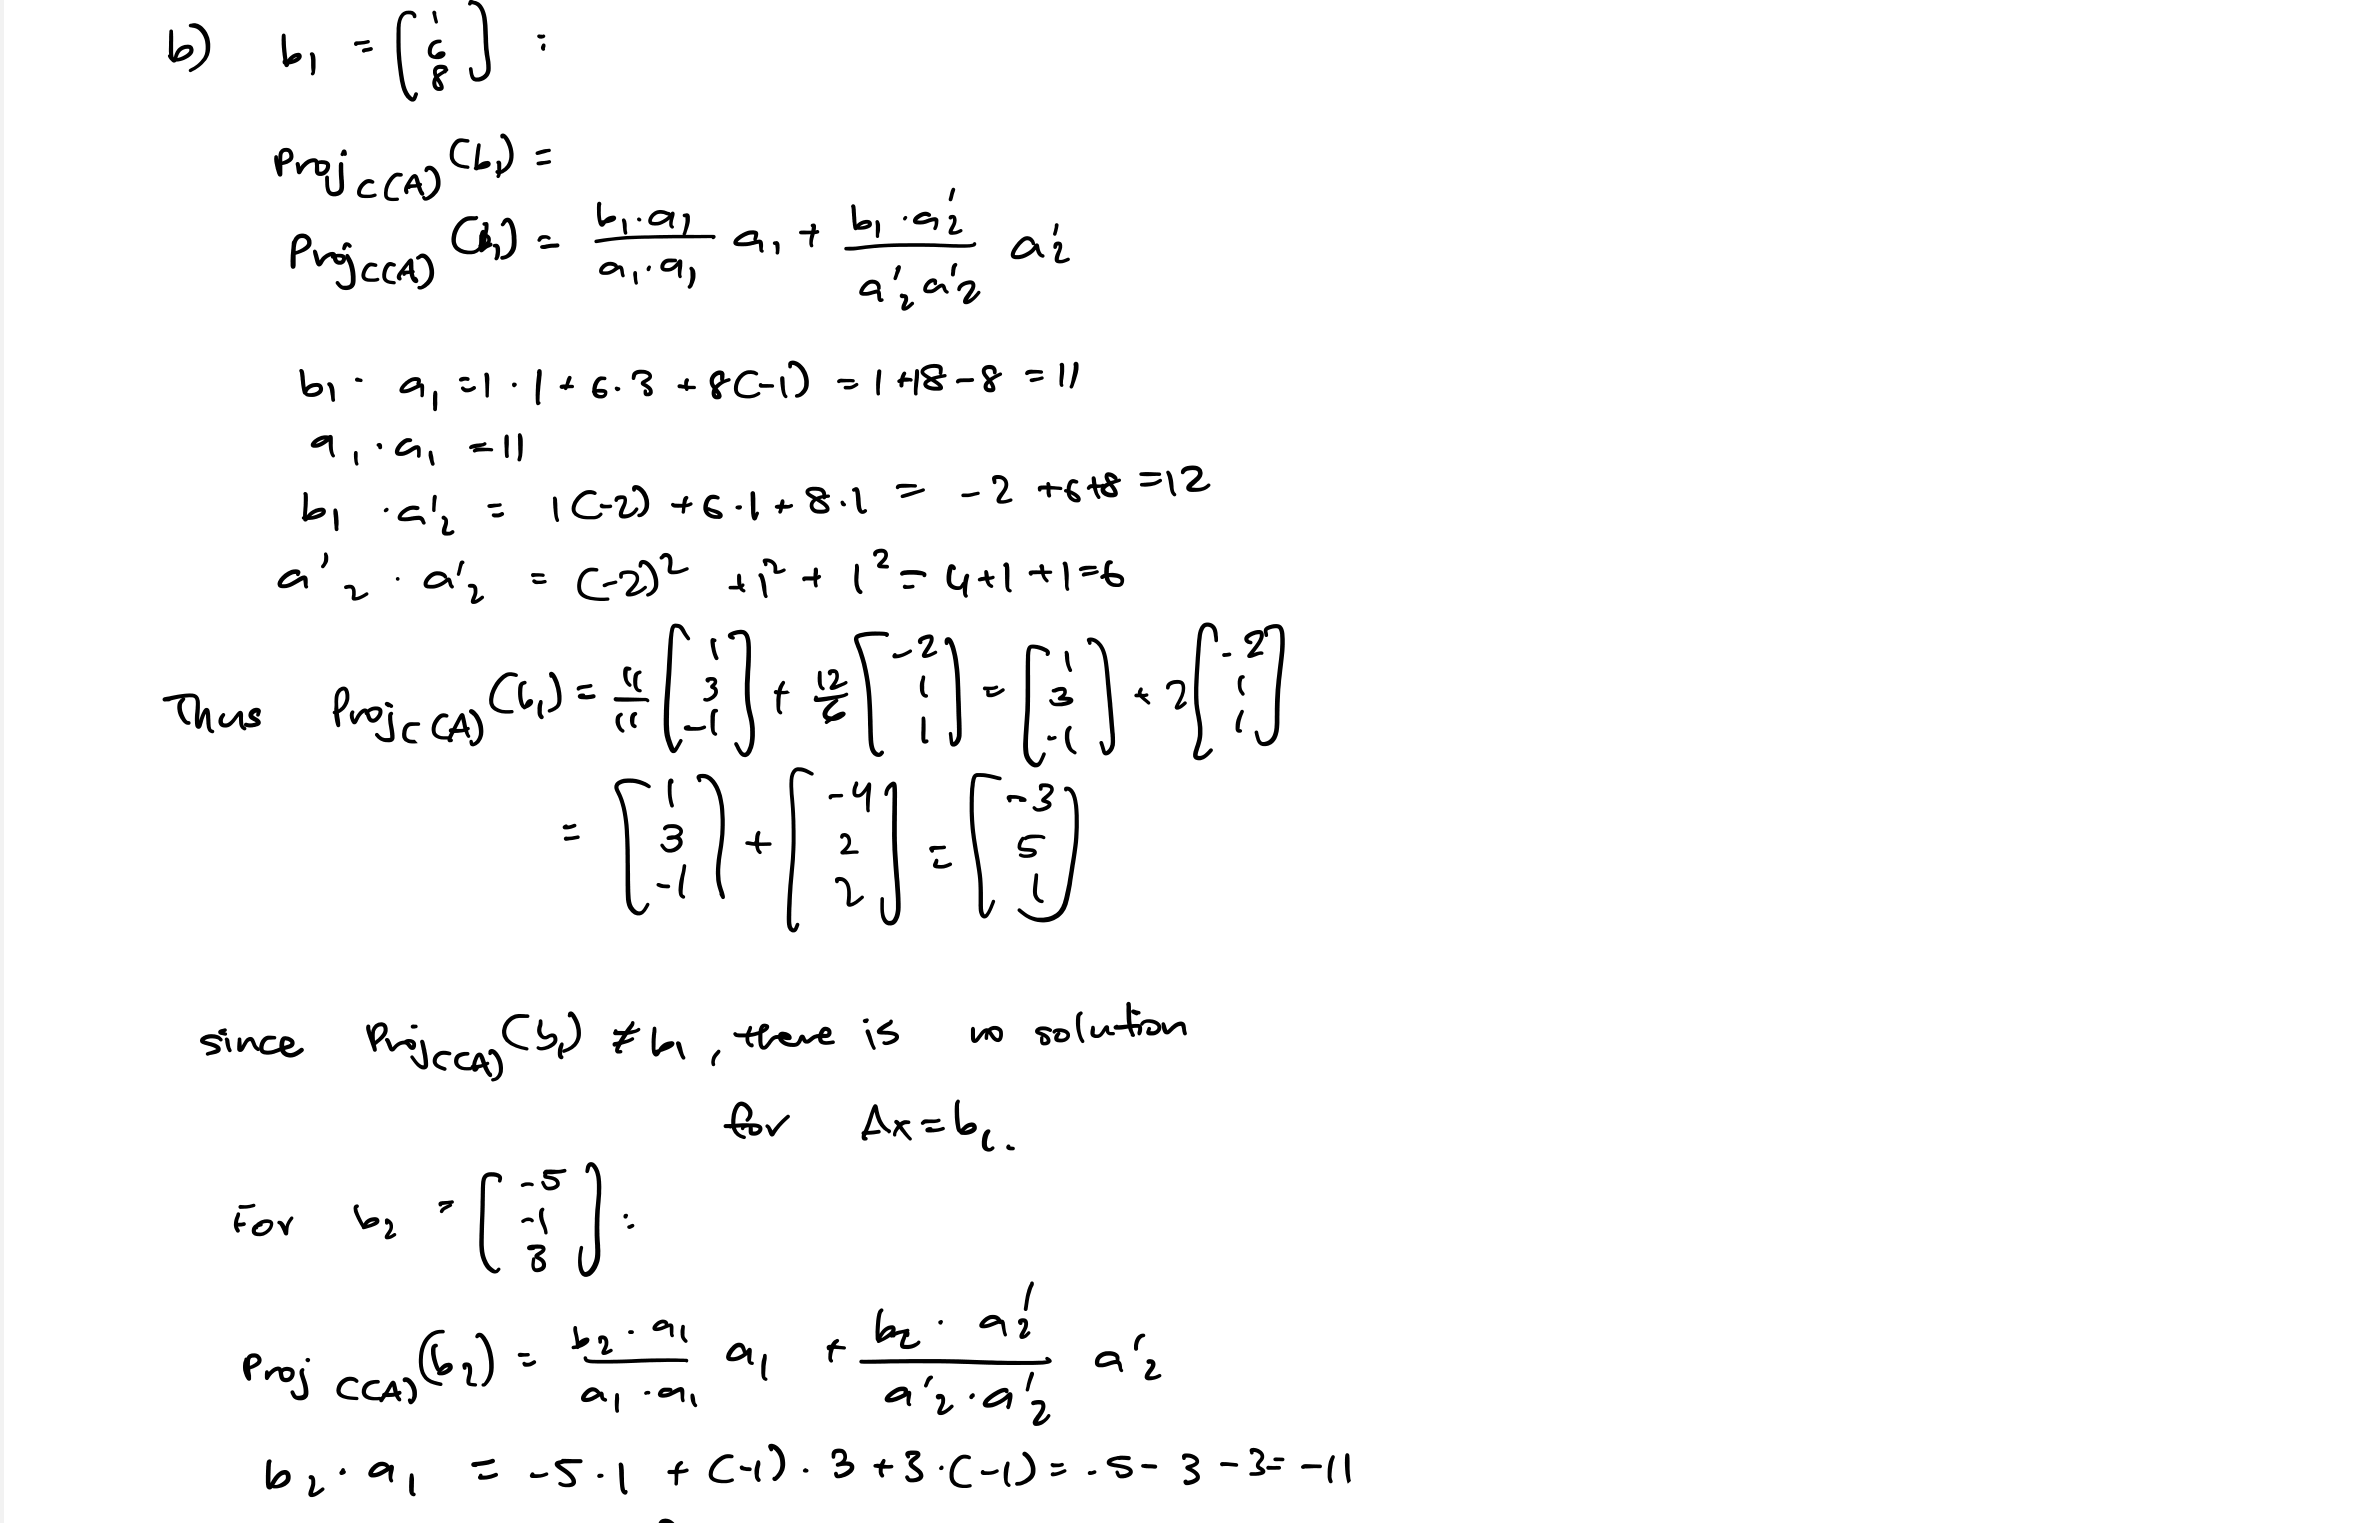
\includegraphics[width=0.8\textwidth]{img1.png}
    \caption{Part b, image 1.}
\end{figure}
\begin{figure}
    \centering
    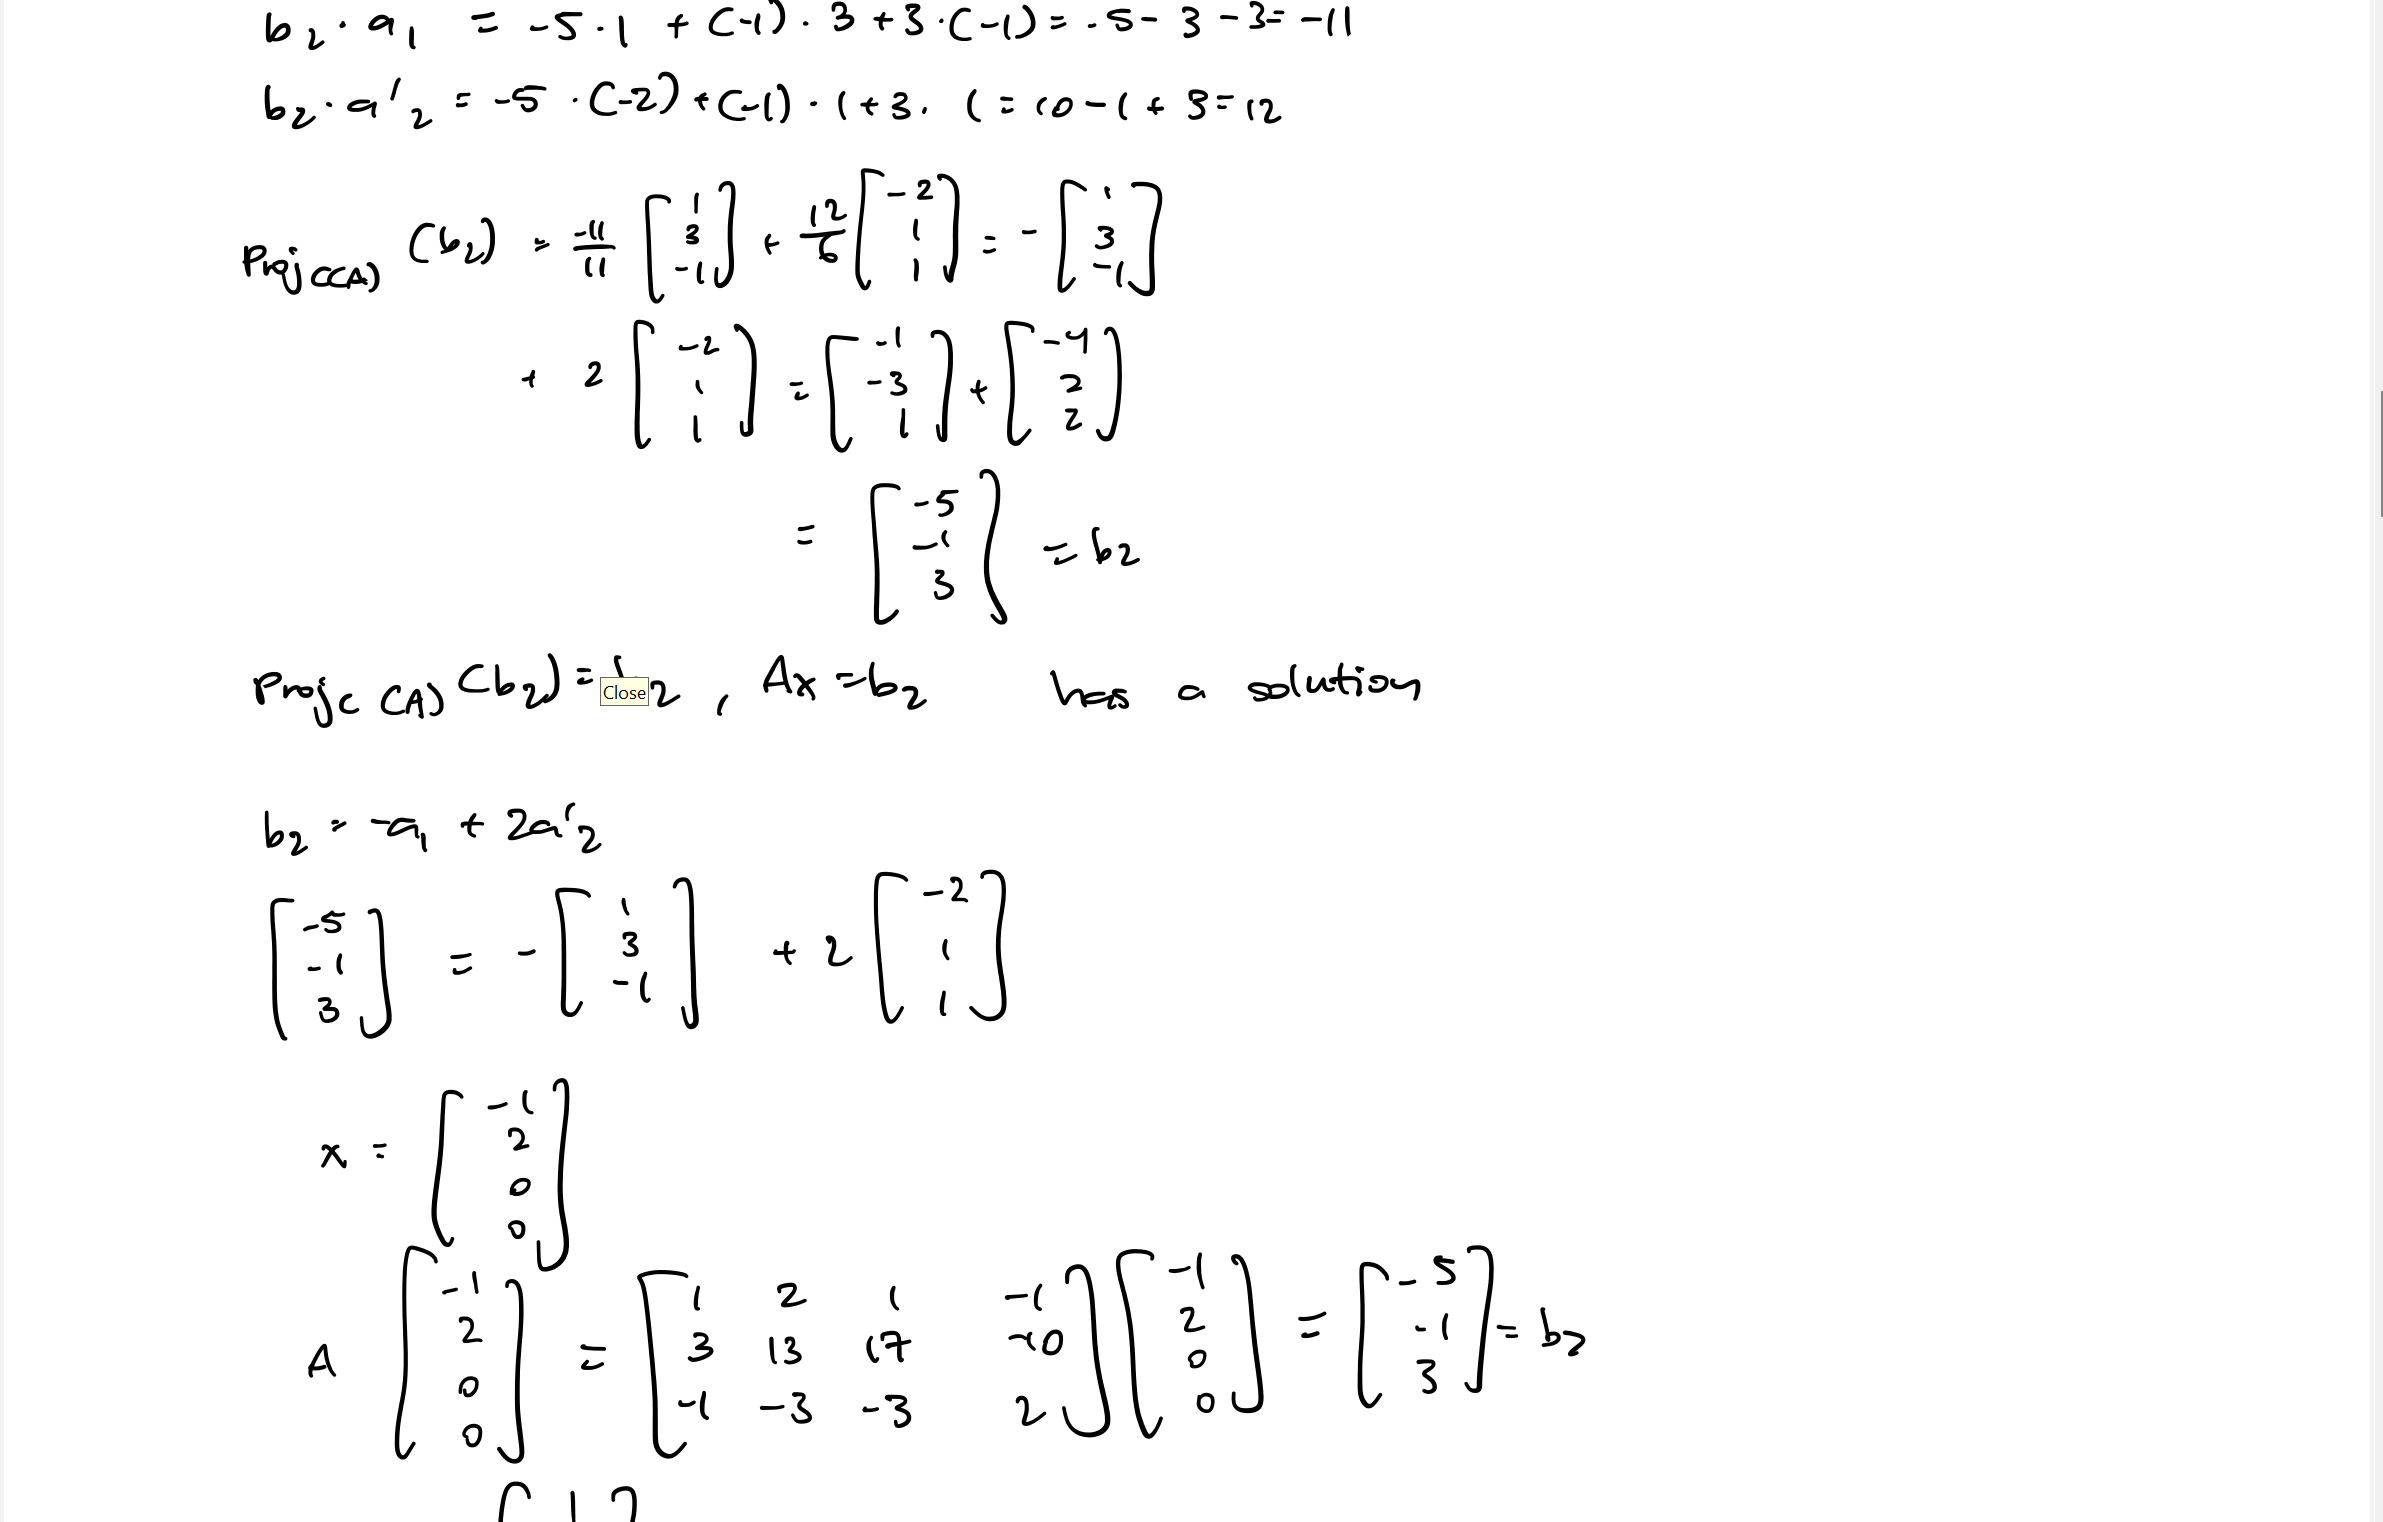
\includegraphics[width=0.8\textwidth]{img2.png}
    \caption{Part b, image 2.}
\end{figure}
\begin{figure}
    \centering
    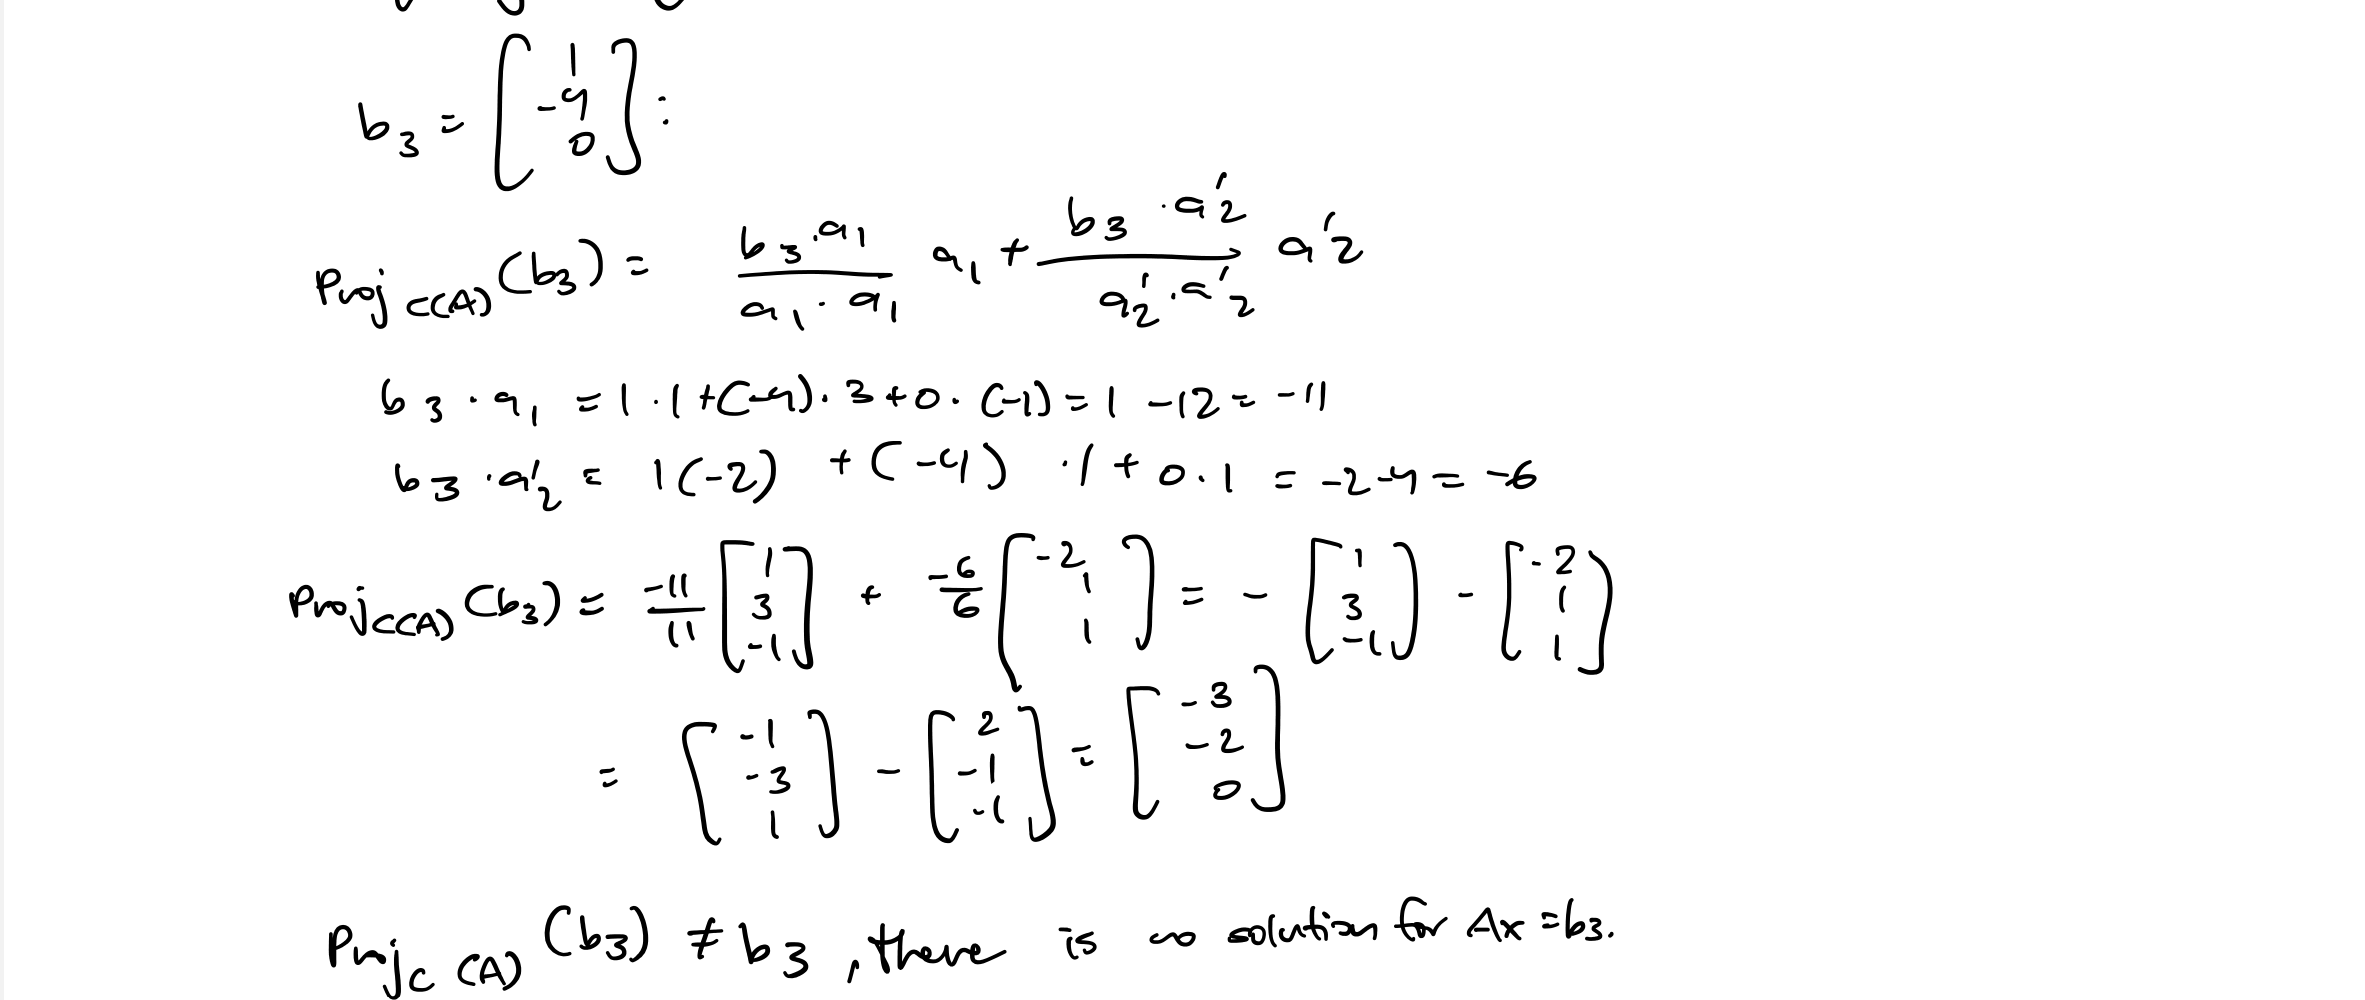
\includegraphics[width=0.8\textwidth]{img3.png}
    \caption{Part b, image 3.}
\end{figure}

\subsection{Parametric Form}

This is completed handwritten.

% Include img4.png
\begin{figure}[ht]
    \centering
    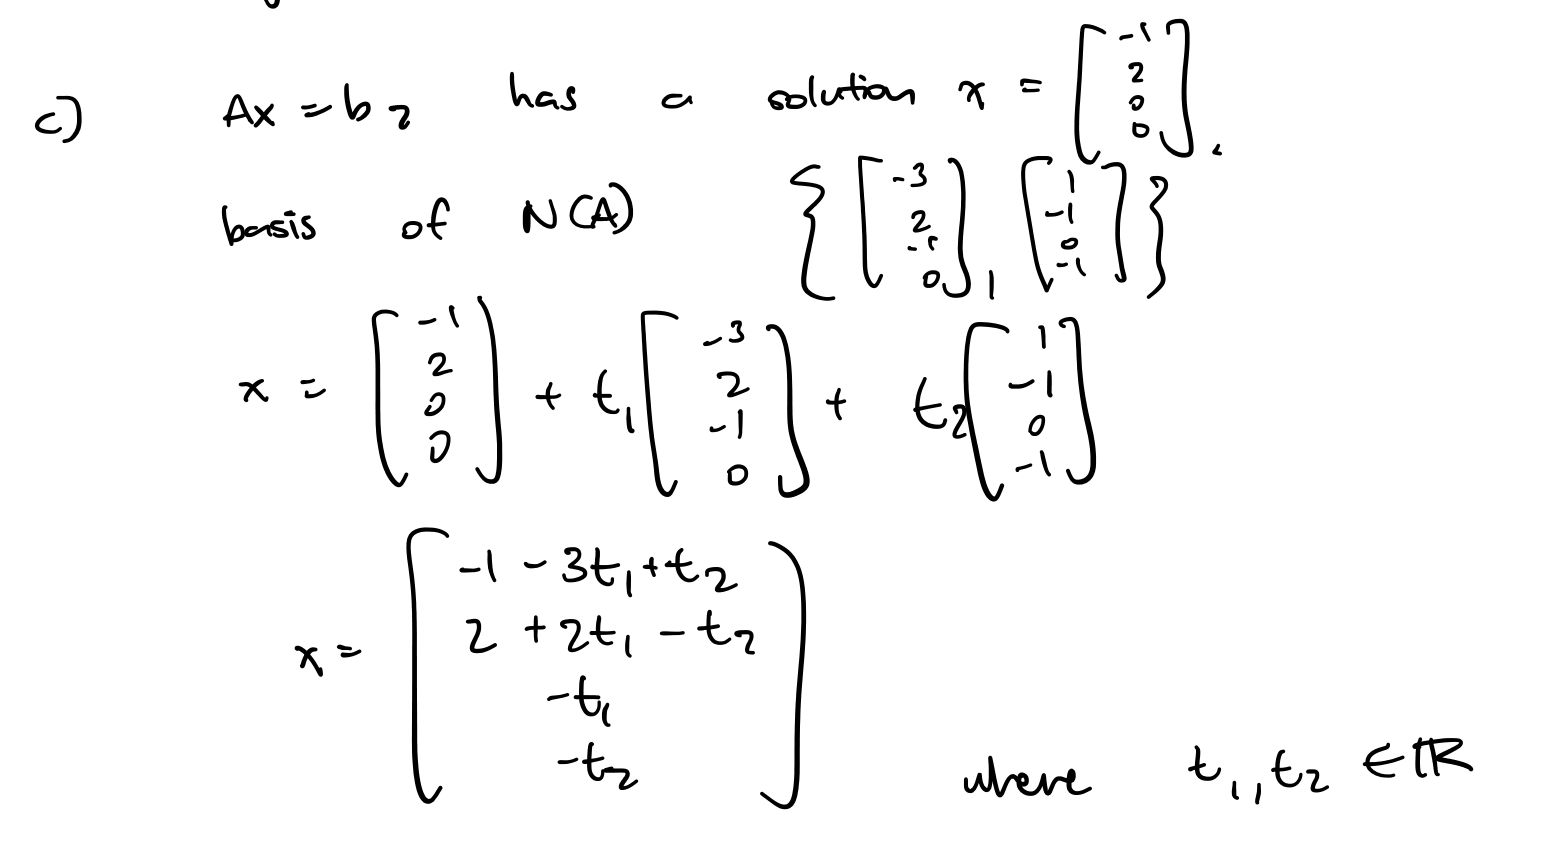
\includegraphics[width=0.8\textwidth]{img4.png}
    \caption{Part c.}
\end{figure}

\end{document}

